%!TEX encoding = UTF-8 Unicode
%!TEX root = ../compendium2.tex

\Lab{\LabWeekEIGHT}

\begin{Goals}
\item Kunna skapa och använda matriser med hjälp av en generisk datatyp.
\item Kunna iterera över alla element i en matris.
\item Träna på algoritmkonstruktion.
\item Träna på hantering av både oföränderliga och förändringsbara objekt.
\item Använda en integrerad utvecklingsmiljö (IDE).
\end{Goals}

\begin{Preparations}
\item Gör övning {\tt \ExeWeekEIGHT} i kapitel \ref{chapter:W08}, speciellt uppgift \ref{exe:matrices:labprep}.

\item Läs appendix \ref{appendix:ide} och välj vilken IDE du ska använda. Säkerställ att du får igång en av dessa utvecklingsmijöer genom att köra hello-world-exemplet och sedan ladda ner och importera kursens \code{workspace} enligt instruktionerna i appendix \ref{appendix:ide}.

\item Läs igenom hela laborationen och studera den befintliga koden i  \code{workspace}.

\end{Preparations}


\begin{figure}[H]
  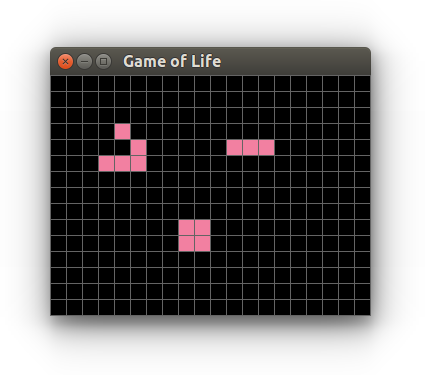
\includegraphics[width=0.8\textwidth]{../img/glider-blinker-block}

  \vspace{-2em}\caption{\label{lab:life:glider-blinker-block}Ett binärt, mörkt datauniversum av dimension $15  \times 20$. Cellkolonin innehåller tre cellgrupper: ett rymdskepp av typen \emph{glider}, en \emph{blinker} och ett \emph{block}.}
\end{figure}


\subsection{Bakgrund}

\emph{Game of Life} simulerar en koloni av encelliga organismer som lever, förökar sig och dör i en matris, enligt några enkla men väl valda regler som konstruerades av matematikern John Horton Conway på 1970-talet. Spelet går ut på att simulera flera generationer utifrån en startkonfiguration, även kallad \emph{cellkoloni}, där varje enskild cells överlevnad beror på dess omgivning. Spelet har inga medvetna spelare och om reglerna följs så kommer slutresultatet enbart bero på startkonfigurationen.

I \emph{Game of Life} består universum av en matris med celler som är antingen levande eller döda. Varje cell har 8 stycken \emph{grannar}, som utgörs av de närmsta omgivande cellerna vertikalt, horisontellt och diagonalt. Varje cells tillstånd i nästa generation bestäms av följande regler:
\begin{enumerate}[nolistsep]
    \item \textbf{Fortlevnad}. Om en levande cell har två eller tre grannar så lever den vidare.
    \item \textbf{Död}. Om en levande cell har mindre än två eller mer än tre grannar så dör den av underpopulation respektive överpopulation.
    \item \textbf{Födelse}. Om cellen är död och har exakt tre grannar så föds den och dess tillstånd ändras till levande, annars fortsätter den vara död.
\end{enumerate}

Flera cellkolonier uppvisar ett ''levande'' beteende där cellmatrisen koloniseras på intressanta vis när en sekvens av generationer visualiseras. Detta är ett exempel på \emph{emergent} beteende där komplexa, självorganiserade strukturer kan uppstå ur enkla förutsättningar.

Läs mer om \emph{Game of Life} på Wikipedia:
\begin{itemize}[noitemsep,topsep=0pt]
    	\item \url{https://en.wikipedia.org/wiki/Conway's_Game_of_Life}
    	\item \url{https://sv.wikipedia.org/wiki/Game_of_Life}
\end{itemize}


\subsection{Obligatoriska krav}

Följande funktionella krav ska uppfyllas av ditt program:
\begin{itemize}[nosep, label={$\square$},]
\item Levande celler ska ha den vackra rosa\footnote{\url{https://www.dsek.se/aktiva/grafiskprofil/farg.php}} RGB-färgen \code{(242, 128, 161)}.
\item Döda celler ska vara svarta som rymden.
\item Detta mörka universum med binära dataceller ska ritas i ett rutnät bestående av smala, stilfulla linjer, så som visas i fig. \ref{lab:life:glider-blinker-block}.
\item Tangenttryckningar och musklick ska fungera enligt följande hjälptext, som ska skrivas ut då programmet startas:
\begin{CodeSmall}
  val help = """
    Welcome to GAME OF LIFE!

    Click on cell to toggle.
    Press ENTER for next generation.
    Press SPACE to toggle play/stop.
    Press R to create random life.
    Press BACKSPACE to clear life.
    Close window to exit.
  """
\end{CodeSmall}
Då \emph{play} aktiveras med blankstegstangenten ska en kontinuerlig simulering av universum fortgå där varje ny generation visualiseras med en lagom fördröjning emellan generationer, tills simuleringen stoppas, t.ex. genom tryck ånyo på blankstegstangenten. Vid varje \emph{Enter}-tryck visas \emph{en} efterkommande generation och ev. pågående simulering stoppas. Vid musklick på en cell ska livstillståndet växlas från levande till död eller vice versa. Ett tryck på R ska ge slumpmässigt liv. Ett tryck på backstegstangenten ska rendera alla universums cellers död.

\end{itemize}

\vspace{1em}\noindent Din kod ska utformas enligt dessa design-krav:
\begin{itemize}[nosep, label={$\square$}]
\item Alla klasser och singelobjekt ska ligga i paketet \code{life}.
\item Det ska finnas en oföränderlig case-klass \code{Life} som representerar ett celluniversum med hjälp av en \code{Matrix[Boolean]} från uppgift \ref{exe:matrices:labprep} i veckans övning.
\item Det ska finnas en klass \code{LifeWindow} som visualiserar en  instans av klassen \code{Life} i ett  \code{introprog.PixelWindow} så som i fig. \ref{lab:life:glider-blinker-block}.
\end{itemize}


\subsection{Valbara krav -- välj minst ett}

Du ska implementera minst ett (gärna flera) av dessa krav:
\begin{itemize}[nosep, label={$\square$}]
\item Cellerna ska färgläggas i olika färger i enlighet med reglerna för nästa generation. Fortlevnad ska fortfarande vara vackert rosa och fortvarig död svart. Följande färger föreslås men välj andra om du tycker det blir finare:
\begin{CodeSmall}
  val UnderPopulated = java.awt.Color.cyan  // en giftig färg
  val OverPopulated  = java.awt.Color.red   // rödklämd av trängsel
  val WillBeBorn     = new java.awt.Color(40, 0, 0)  // snart levande
\end{CodeSmall}
Ge \code{LifeWindow} en klassparameter \code{isMultiColor} som styr om det blir mångfärgade celler eller om det bara finns rosa och svart som i grundkraven.

\item Om man trycker på \code{S} för \emph{Save} ska \code{introprog.Dialog.file("Save Life")} visas och, om användaren inte trycker \Button{Cancel}, det aktuella livet sparas med hjälp av \code{introprog.IO.saveString} i en textfil via metoden \code{toString} i \code{Life}.

\item Om man trycker på \code{O} för \emph{Open} ska \code{introprog.Dialog.file("Open Life")} anropas och ett nytt universum läsas in från textfil enligt lämpligt format. Inläsningen ska ske med hjälp av \code{introprog.IO.loadString} och tolkas till en \code{Life}-instans av en metod i kompanjonsobjektet med detta huvud:
\begin{CodeSmall}
def fromString(s: String, rowDelim: String="\n", alive: Char='0'): Life
\end{CodeSmall}
Testa med filen \texttt{glider-gun.txt} som ska ha följande innehåll på de första 11 raderna och totalt 32 rader där alla rader efter elfte raden innehåller tomt liv:
\begin{REPLnonum}
> head -11 glider-gun.txt
------------------------------------------
-------------------------0----------------
-----------------------0-0----------------
-------------00------00------------00-----
------------0---0----00------------00-----
-00--------0-----0---00-------------------
-00--------0---0-00----0-0----------------
-----------0-----0-------0----------------
------------0---0-------------------------
-------------00---------------------------
------------------------------------------
\end{REPLnonum}
\item Universum ska vara cirkulärt, d.v.s grannen vid kanten finns på andra sidan genom att indexeringen börjar om \Eng{wrapped} enligt modulo-räkning. Inför en klassparameter \code{isWrapped} i \code{Life} och en variabel \code{wrapped: Boolean} i kompanjonsobjektet \code{Life} som styr om fabriksmetoderna skapar ett universum som är cirkulärt eller ej, så att du lätt kan konfigurera detta. \emph{Tips:} Du har stor nytta av att använda \code|java.lang.Math.floorMod| i \code{apply}-metoden i \code{Life}; metoden \code{floorMod} räknar på lämpligt sätt med negativa värden, se dokumentationen för \code{Math}-paketet i JDK8.

\item Läs om varianter till \code{Game of Life} på Wikipedia och implementera alternativa regler som görs valbara genom konfigurering via \code{args}-parametern i \code{main}.

\item Skapa en klass \code{LifeStatistics} som genom väldigt många simuleringar ska ta reda på sannolikheten att en slumpmässig cellkoloni efter $n$ generationer fortfarande utvecklas, respektive är helt dött. Ingen visualisering med \code{PixelWindow} ska ske; endast antalet celler som lever vid generation $n$ och antalet celler som ändrades sedan generation $n - 1$ behöver registreras.

\end{itemize}




\subsection{Tips och förslag}

\begin{enumerate}[leftmargin=*]
\item Här är ett förslag på hur du kan utforma klassen \code{Life}:
\scalainputlisting[basicstyle=\ttfamily\fontsize{10}{12}\selectfont]{../workspace/w08_life/src/main/scala/life/Life.scala}
% \begin{CodeSmall}
% package life
%
% case class Life(cells: Matrix[Boolean]) {
%
%   /** Ger true om cellen på plats (row, col) är vid liv annars false.
%     * Ger false om indexeringen är utanför universums gränser.
%     */
%   def apply(row: Int, col: Int): Boolean = ???
%
%   /** Sätter status på cellen på plats (row, col) till value. */
%   def updated(row: Int, col: Int, value: Boolean): Life = ???
%
%   /** Växlar status på cellen på plats (row, col). */
%   def toggled(row: Int, col: Int): Life = ???
%
%   /** Räknar antalet levande grannar till cellen i (row, col).*/
%   def nbrOfNeighbours(row: Int, col: Int): Int = ???
%
%   /** Skapar en ny Life-instans med nästa generation av universum.
%     * Detta sker genom att applicera funktionen \code{rule} på cellerna.
%     */
%   def evolved(rule: (Int, Int, Life) => Boolean = Life.defaultRule):Life = {
%     var nextGeneration = Life.empty(cells.dim)
%     cells.foreachIndex { (r,c) =>
%       ???
%     }
%     nextGeneration
%   }
%
%   override def toString =
%     cells.data.map(_.map(if (_) '0' else '-').mkString).mkString("\n")
% }
%
% object Life {
%   /** Skapar ett universum med döda celler. */
%   def empty(dim: (Int, Int)): Life = ???
%
%   /** Skapar ett unviversum med slumpmässigt liv. */
%   def random(dim: (Int, Int)): Life = ???
%
%   /** Implementerar reglerna enligt Conways Game of Life. */
%   def defaultRule(row: Int, col: Int, current: Life): Boolean = ???
% }
% \end{CodeSmall}
Du har nytta av metoden \code{nbrOfNeighbours} när du ska implementera \code{defaultRule}. Vid implementation av \code{random} är metoden \code{foreachIndex} i \code{Matrix[T]} smidig att använda.
Om du som i förslaget ovan låter \code{evolved} ta uppdateringsregeln som en funktionsparameter blir det lättare att konfigurera vilka regler som ska gälla och därmed blir det även lättare att skapa varianter av \emph{Game of Life} genom att införa nya regler i kompanjonsobjektet (se en av de valfria uppgifterna med vidare hänvisning till Wikipedia).

\item Här är ett förslag på hur du kan utforma klassen \code{LifeWindow}:
\scalainputlisting[basicstyle=\ttfamily\fontsize{10}{12}\selectfont]{../workspace/w08_life/src/main/scala/life/LifeWindow.scala}
% \begin{CodeSmall}
% package life
%
% import introprog.PixelWindow
% import introprog.PixelWindow.Event
%
% class LifeWindow(rows: Int, cols: Int){
%   import LifeWindow._ // importera konstanter för cellstorlek, färger, etc.
%
%   var life = Life.empty(rows, cols)
%   val window: PixelWindow = ???
%   var quit = false
%   var play = false
%
%   def drawGrid(): Unit = ???
%
%   def drawCell(row: Int, col: Int): Unit = ???
%
%   def update(newLife: Life): Unit = {
%     val oldLife = life
%     life = newLife
%     life.cells.foreachIndex{ ??? }
%   }
%
%   def handleKey(key: String): Unit = ???
%
%   def handleClick(pos: (Int, Int)): Unit = ???
%
%   def loopUntilQuit(): Unit = while (!quit) {
%     val t0 = System.currentTimeMillis
%     if (play) update(life.evolved())
%     window.awaitEvent(EventMaxWait)
%     while (window.lastEventType != PixelWindow.Event.Undefined) {
%       window.lastEventType match {
%         case Event.KeyPressed  =>  handleKey(window.lastKey)
%         case Event.MousePressed => handleClick(window.lastMousePos)
%         case Event.WindowClosed => quit = true
%         case _ =>
%       }
%       window.awaitEvent(EventMaxWait)
%     }
%     val elapsed = System.currentTimeMillis - t0
%     Thread.sleep((NextGenerationDelay - elapsed) max 0)
%   }
%
%   def start(): Unit = { drawGrid(); loopUntilQuit() }
% }
% \end{CodeSmall}

\item \textbf{Dra nytta av den IDE du valt.} Det finns många användbara finesser i en integrerad utvecklingsmiljö. Orientera dig om grunderna genom att läsa appendix \ref{appendix:ide}. Lär dig några viktiga kortkommandon och studera hur du får igång debuggern. Prova att i debuggern sätta brytpunkter, stega dig fram och avläsa variablers värden.
\end{enumerate}
